%\documentclass{article}
\documentclass[UTF8]{ctexart}
% Language setting
% Replace `english' with e.g. `spanish' to change the document language
\usepackage[english]{babel}
\usepackage{amsmath}
% Set page size and margins
% Replace `letterpaper' with `a4paper' for UK/EU standard size
\usepackage[a4paper,top=2cm,bottom=2cm,left=3cm,right=3cm,marginparwidth=1.75cm]{geometry}

% Useful packages
\usepackage{amsmath}
\usepackage{graphicx}
\usepackage[colorlinks=true, allcolors=blue]{hyperref}

\title{曲线积分与路径无关}
\author{Bright Moon}

\begin{document}
\maketitle
\section{曲线积分与路径无关的相关表述}
\[\int _L \vec F(x,y,z) \cdot d\vec r\]
其中,$L$是区域$D$中的一条有向路径;$\vec F(x,y,z)$ 是一个三元向量函数。
\[\vec F(x,y,z) = (P(x,y,z),Q(x,y,z),R(z,y,z))\]
\begin{enumerate}
    \item 第二型曲线积分与路径无关。
    \item $\vec F(x,y,z)$在$D$内是保守场。
    \item $\vec F(x,y,z)$在$D$内沿任意闭曲线$\Gamma$环量为零。\[\oint _{\Gamma} \vec F(x,y,z)\cdot d\vec r = 0\]
    \item $\vec F(x,y,z)$在$D$内存在连续可微的原函数$f(x,y,z)$。
    \item $\vec F(x,y,z)$在$D$内可以看作一个函数$u(x,y,z)$的负梯度。\[\vec F(x,y,z) = -\nabla u(x,y,z)\]
    \item $\vec F(x,y,z)$在$D$内是有势场。
    \item $\vec F(x,y,z)$在$D$内是无旋场。\[\nabla \times \vec F(x,y,z) = \vec 0\]
    \item 
        $\frac{\partial R}{\partial y}=\frac{\partial Q}{\partial z}$;$\frac{\partial P}{\partial z}=\frac{\partial R}{\partial x}$;$\frac{\partial Q}{\partial x}=\frac{\partial P}{\partial y}$
\end{enumerate}
\section{相关表述的等价性}
\subsection{紧凑的表示}
\begin{equation}
    1\Leftrightarrow 2\Leftrightarrow 3\Leftrightarrow 4\Leftrightarrow 5\Leftrightarrow 6\begin{cases}
    \longrightarrow 7\Leftrightarrow 8,\quad \text{不要求$D$单连通}\\
    \longleftarrow 7\Leftrightarrow 8,\quad \text{要求$D$单连通}
    \end{cases}
\end{equation}
\subsection{文字描述}
1是2的定义,5是6的定义。1、2、3、4、5、6彼此之间两两等价。根据旋度的定义,7、8等价。
\par
根据旋度的定义(旋度取环量面密度最大的数值与方向),3可以推出7。类似的,由于连续函数混合偏导数相等,所以4可以推出8。这两条向右走的逻辑都不需要$D$为单连通区域。
\par
7推出3要借助斯托克斯公式,因此,要求$D$是单连通区域。
\[\oint _{\partial S} \vec F(x,y,z)\cdot d\vec r = \iint_S \left(\nabla \times \vec F(x,y,z) \right) \cdot d\vec S\]
斯托克斯公式可以在多连通区域使用。但是只有在单连通区域,$\Gamma$才可能是双侧曲面$S$的边界,即,$\Gamma = \partial S$。

\begin{figure}
    \centering
    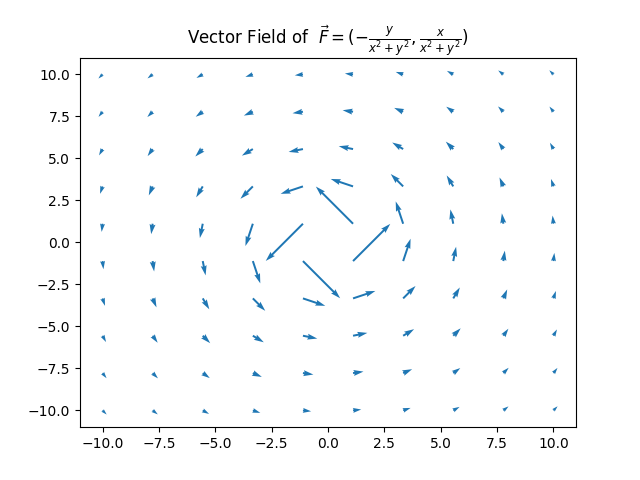
\includegraphics[width=0.75\linewidth]{Figure_1.png}
\end{figure}











\end{document}